\documentclass{beamer}
% \usepackage{beamerthemesplit}
\usetheme{Madrid}
% \usepackage{pstricks}
\usepackage{graphicx}
\usepackage{mdwlist}
\usepackage{lineno, hyperref}
\usepackage{stackrel}
\usepackage{changepage}

\usepackage{amssymb,latexsym,amsmath,amsthm,bbm}
\usepackage{hyperref}
\usepackage{tikz}
\usepackage[english]{babel}
\usepackage[latin1]{inputenc}
\usepackage[authoryear]{natbib}
\usepackage{multirow}
\usepackage{verbatim}
\usepackage{alltt}
\usepackage{mycommands}

% \usepackage{cmbright}
\renewcommand*\familydefault{\sfdefault}
\usepackage[T1]{fontenc}


\definecolor{wp-red}{RGB}{204,0,0}
\definecolor{wp-gray}{RGB}{51,51,51}
\definecolor{reynolds-red}{RGB}{153,0,0}
\definecolor{pyroman-flame}{RGB}{209,81,34}
\definecolor{hunt-yellow}{RGB}{253,215,38}
\definecolor{genomic-green}{RGB}{125,140,31}
\definecolor{innovation-blue}{RGB}{66,126,147}
\definecolor{bio-indigo}{RGB}{65,86,161}

\setbeamercolor{structure}{fg=wp-red}
\setbeamercolor{title}{bg=white, fg=wp-red}  % changes color on title page
\setbeamerfont{title}{series=\bfseries, size=\huge}
\setbeamerfont{author}{series=\bfseries, size=\large}
\setbeamerfont{institute}{series=\mdseries, size=\large}

\setbeamercolor{frametitle}{bg=wp-red, fg=white}  % changes color at top of frame
\setbeamerfont{frametitle}{series=\bfseries}
\setbeamercolor{title in head/foot}{fg=white, bg=wp-red}  % changes color for title in footer
\setbeamerfont{title in head/foot}{series=\bfseries}
\setbeamercolor{author in head/foot}{fg=white,bg=wp-gray}  % changes color for author in footer
\setbeamerfont{author in head/foot}{series=\bfseries}

\title[Spatial methods for EVA] % (optional, use only with long paper titles)
{
  Spatial methods for extreme value analysis
}
\author[S. Morris]{Samuel A. Morris}
% \institute[]{North Carolina State University}
\date[]{17 Mar 2016}

\begin{document}

\begin{frame}\frametitle{\ }
\begin{center}
  \maketitle
\end{center}
\end{frame}

\begin{frame}{Motivation}
  \begin{itemize} \setlength{\itemsep}{1em}
    \item Average behavior is important to understand, but it does not paint the whole picture
    \begin{itemize}
      \item e.g. When constructing river levees, engineers need to be able to estimate a 100-year or 1000-year flood levels
      \item e.g. Probability of ambient air pollution exceeding a certain threshold level
    \end{itemize}
    \item Estimating the probability of rare events is challenging because these events are, by definition, rare
    \item Spatial extremes is promising because it borrows information across space
    \item Spatial extremes is also useful for estimating probability of extremes at sites without data
  \end{itemize}
\end{frame}

\begin{frame}{Defining extremes}
\begin{columns}[c]
\column{.45 \linewidth}
  \begin{itemize} \setlength{\itemsep}{1em}
    \item Key in extreme value analysis is to define extremes
    \item Typically done in one of two ways
    \begin{itemize}
      \item Block maxima (red dots)
      \item Values over threshold considered extreme
    \end{itemize}
  \end{itemize}

  \column{.55\linewidth}
  \begin{figure}
    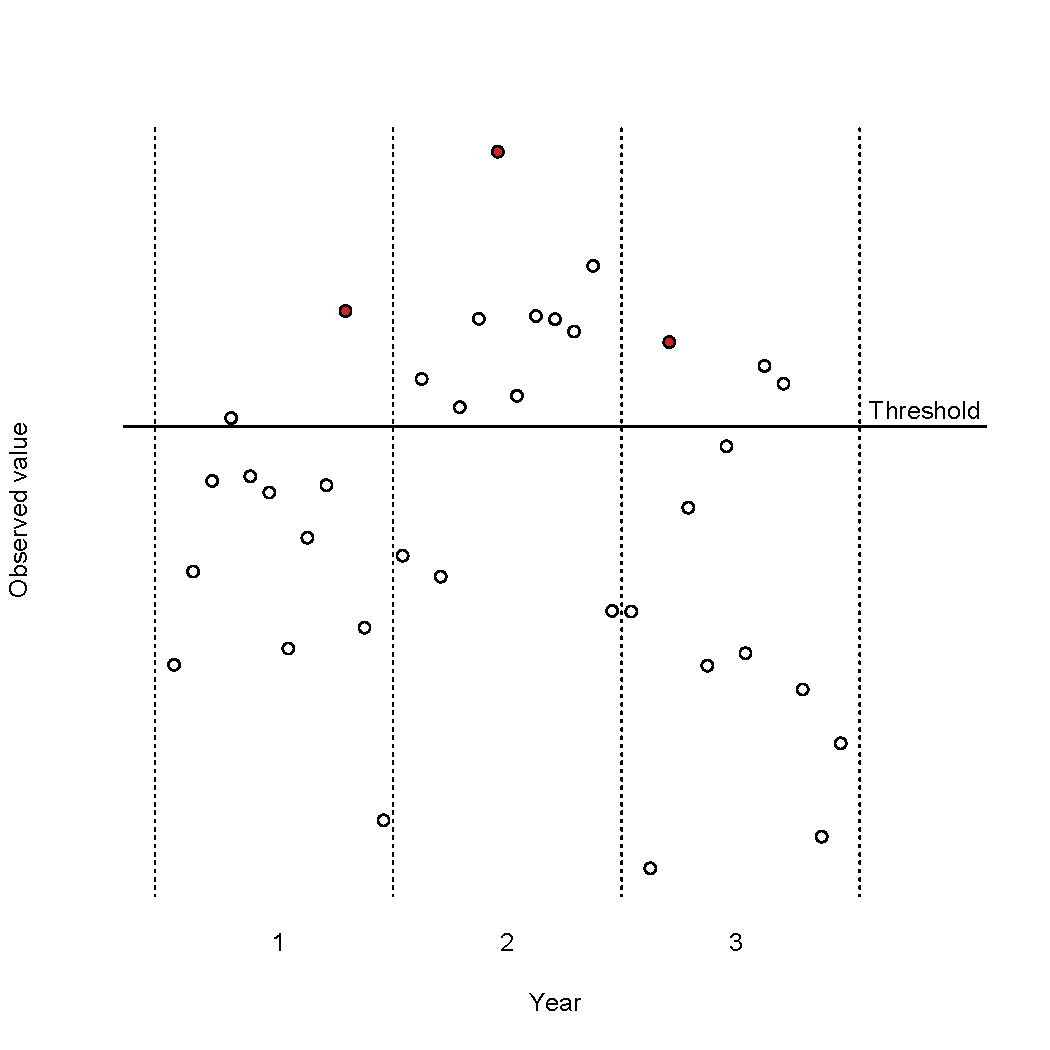
\includegraphics[width=1\linewidth, trim=0 0.5in 0 1in]{./plots/define_extreme.pdf}
    \caption{Hypothetical monthly data}
    \end{figure}
\end{columns}
\end{frame}

\begin{frame}{Non-spatial analysis: Block maxima}
\begin{adjustwidth}{1em}{0em}
  Fisher-Tippett-Gnedenko theorem \vspace{1em}
  \begin{itemize} \setlength{\itemsep}{1em}
    \item Let $X_1, \ldots, X_n$ be i.i.d.
    \item Consider the block maximum $M_n = \max(X_1, \ldots, X_n)$
    \item If there exist normalizing sequences $a_n > 0$ and $b_n \in \calR$ such that
    \begin{align*}
      \frac{ M_n - b_n }{ a_n } \converged G(z)
    \end{align*}
    then $G(z)$ follows a generalized extreme value distribution (GEV) (Gnedenko, 1943)
    \item This motivates the use of the GEV for block maximum data
  \end{itemize}
\end{adjustwidth}
\end{frame}

\begin{frame}{Non-spatial analysis: Block maxima}
  \begin{itemize} \setlength{\itemsep}{1em}
    \item GEV distribution
    \begin{align*}
      G(y) = \Pr(Y < y) = \left\{  \begin{array}{ll}
        \exp\left\{ -\left[ 1 + \xi \left( \frac{ y - \mu }{ \sigma } \right) \right]^{ -1 / \xi} \right\} & \quad \xi \neq 0 \\[0.5em]
        \exp \left\{ -\exp \left( - \frac{ y - \mu }{ \sigma} \right) \right\} & \quad \xi = 0
      \end{array}\right.
    \end{align*}
    where
    \begin{itemize} \setlength{\itemsep}{0.25em}
      \item $\mu \in \calR$ is a location parameter
      \item $\sigma > 0$ is a scale parameter
      \item $\xi \in \calR$ is a shape parameter
      \begin{itemize}
        \item Unbounded above if $\xi \ge 0$
        \item Bounded above by $(\mu - \sigma) / \xi$ when $\xi < 0$
      \end{itemize}
    \end{itemize}
    \item Challenges:
    \begin{itemize}
      \item Lose information by only considering maximum in a block
      \item Underlying data may not be i.i.d.
    \end{itemize}
  \end{itemize}
\end{frame}

\begin{frame}{Non-spatial analysis: Peaks over threshold}
\begin{adjustwidth}{1em}{0em}
  Pickands-Balkema-de Haan theorem \vspace{1em}
  \begin{itemize} \setlength{\itemsep}{1em}
    \item Let $X_1, \ldots, X_n \iid F$
    \item If there exist normalizing sequences $a_T > 0$ and $b_T \in \calR$ such that for any $x \ge 0$, as $T \rightarrow \infty$
    \begin{align*}
      \Pr\left(\frac{X - b_T}{a_T} > x \mid X > T\right) \converged H(x),
    \end{align*}
    where $T$ is a thresholding value, then $H(x)$ follows a generalized Pareto distribution (GPD) (Balkema and de Haan, 1974)
  \end{itemize}
\end{adjustwidth}
\end{frame}

\begin{frame}{Non-spatial analysis: Peaks over threshold}
\begin{adjustwidth}{1em}{0em}
  Select a threshold, $T$, and use the GPD to model the exceedances
  \begin{align*}
    H(y) = P(Y < y) = \left\{ \begin{array}{ll}
      1 - \left[1 - \xi \left( \frac{ y - T }{ \sigma } \right) \right]^{-1 / \xi} & \quad \xi \neq 0 \\[0.5em]
      1 - \exp \left\{ \frac{ y - T }{ \sigma} \right\} & \quad \xi = 0
    \end{array}\right.
  \end{align*}
  where
  \begin{itemize} \setlength{\itemsep}{0.25em}
    \item $\sigma > 0$ is a scale parameter
    \item $\xi \in \calR$ is a shape parameter
    \begin{itemize}
      \item Unbounded above if $\xi \ge 0$
      \item Bounded above by $(T - \sigma) / \xi$ when $\xi < 0$
    \end{itemize}
    \item Challenges: \vspace{0.5em}
    \begin{itemize} \setlength{\itemsep}{0.5em}
      \item Sensitive to threshold selection
      \item Temporal dependence between observations (e.g. flood levels don't dissipate overnight)
    \end{itemize}
  \end{itemize}
\end{adjustwidth}
\end{frame}

% \begin{frame}{Non-spatial analysis: Peaks over threshold}
%   \begin{itemize} \setlength{\itemsep}{1em}
%     \item The GPD is related to GEV distribution through
%     \begin{align*}
%       H(y) = 1 + \log[G(y)], \quad y \ge T
%     \end{align*}
%     \item Challenges: \vspace{0.5em}
%     \begin{itemize} \setlength{\itemsep}{0.5em}
%       \item Sensitive to threshold selection
%       \item Temporal dependence between observations (e.g. flood levels don't dissipate overnight)
%     \end{itemize}
%   \end{itemize}
% \end{frame}

\begin{frame}{Max-stable processes for spatial data}
  \begin{itemize} \setlength{\itemsep}{1em}
    \item Consider i.i.d. spatial processes $x_j(\bs)$, $j = 1, \ldots, J$
    \item Let $M_J(\bs) = \bigvee_{j=1}^J x_j(\bs_i)$ be the block maximum at site $\bs$
    \item If there exists normalizing sequences $a_J(\bs)$ and $b_J(\bs)$ such that for all sites, $\bs_i, i = 1, \ldots, d$,
    \begin{align*}
      \frac{M_J(\bs) - b_J(\bs)}{a_J(\bs)} \converged G(\bs)
    \end{align*}
    then $G(\bs)$ is a max-stable process (Smith, 1990)
    \item Therefore, max-stable processes are the standard model for block maxima
  \end{itemize}
\end{frame}

\begin{frame}{Multivariate representations}
  \begin{itemize} \setlength{\itemsep}{1em}
    \item Marginally at each site, observations follow a GEV distribution
    \item For a finite collection of sites the representation for the multivariate GEV (mGEV) is
    \begin{align*}
      \Pr(\bZ \le \bz)  &= G^*(\bz) = \exp[-V(\bz)]\\
            V(\bz)    &= d \int_{\Delta_d} \bigvee_{i = 1}^d \frac{w_i}{z_i} H(\ddd w)
    \end{align*}
    where
    \begin{itemize} \setlength{\itemsep}{0.25em}
      \item $V(\bz)$ is called the exponent measure
      \item $\Delta_d = \{ \bw \in \calR^d_+ \mid w_1 + \cdots + w_d = 1\}$
      \item $H$ is a probability measure on $\Delta_d$
      \item $\int_{\Delta_d}w_i H(\ddd w) = 1 / d$ for $i = 1, \ldots, d$
    \end{itemize}
  \end{itemize}
\end{frame}

\begin{frame}{Multivariate GEV challenges}
  \begin{itemize} \setlength{\itemsep}{1em}
    \item Only a few closed-form expressions for $V(\bz)$ exist
    \item Two common forms for $V(\bz)$
    \begin{itemize}
      \item Symmetric logistic (Gumbel, 1960)
      \begin{align*}
        V(\bz) = \left[\sum_{i = 1}^n \left( \frac{ 1 }{ z_i } \right)^{1/\alpha}\right]^\alpha
      \end{align*}
      \item Asymmetric logistic (Coles and Tawn, 1991)
      \begin{align*}
        V(\bz) = \sum_{l = 1}^L \left[\sum_{i = 1}^n \left(\frac{w_{il}}{z_i} \right)^{1 / \alpha_l} \right]^{\alpha_l}
      \end{align*}
      where $w_{il} \in [0, 1]$ and $\sum_{l = 1}^L w_{il} = 1$
    \end{itemize}
  \end{itemize}
\end{frame}

\begin{frame}{Multivariate peaks over threshold}
  \begin{itemize} \setlength{\itemsep}{1em}
    \item Few existing methods
    \item Often use max-stable methods due to the relationship between GEV and GPD
    \item Joint distribution function given by Falk et al. (2011)
    \begin{align*}
      H(\bz) = 1 - V(\bz)
    \end{align*}
    where $V(\bz)$ is defined as in the GEV
  \end{itemize}
\end{frame}

\begin{frame}{Extremal dependence: $\chi$ statistic}
  \begin{itemize} \setlength{\itemsep}{1em}
    \item Correlation is the most common measure of dependence
    \begin{itemize}
      \item Focuses on the center and not tails
      \item This makes it irrelevant for extreme value analysis
    \end{itemize}
    \item Extreme value analysis focuses on the $\chi$ statistic (Coles et al., 1999), a measure of extremal dependence given by
    \begin{align*}
      \chi(h) = \lim_{c \rightarrow \infty}\Pr[Y(\bs) > c \mid Y(\bt) > c]
    \end{align*}
    where $h = ||\bs - \bt||$
    \item If $ \chi(h) = 0$, then observations are asymptotically independent at distance $h$
  \end{itemize}
\end{frame}

\begin{frame}{Existing challenges}
  \begin{itemize} \setlength{\itemsep}{1em}
    \item Multivariate max-stable and GPD models have nice features, but they are
    \begin{itemize}
      \item Computationally challenging (e.g,  the asymmetric logistic has $2^{n-1}(n + 2) - (2n + 1)$ free parameters)
      \item Joint density only available in low dimensions
    \end{itemize}
    \item Some recent approaches
    \begin{itemize}
      \item Bayesian hierarchical model (Reich and Shaby, 2012)
      \item Pairwise likelihood approach (Huser and Davison, 2014)
    \end{itemize}
    \item Many opportunities to explore new methods
  \end{itemize}
\end{frame}

% \begin{frame}{Gaussian spatial model}
%   \begin{itemize} \setlength{\itemsep}{1em}
%     \item In geostatistics, $Y(\bs)$ are often modeled using a Gaussian process with mean function $\mu(\bs)$ and covariance function $\rho(h)$
%     \item Model properties
%     \begin{itemize}
%       \item Nice computing properties (closed-form likelihood)
%       \item For a Gaussian spatial model $\chi(h) = 0$ regardless of the strength of the correlation in the bulk of the distribution
%       \item Tail is not flexible
%       \begin{itemize}
%         \item Light-tailed
%         \item Symmetric
%       \end{itemize}
%     \end{itemize}
%   \end{itemize}
% \end{frame}

\begin{frame}{Max-stable processes: A hierarchical representation (Reich \& Shaby, 2012)}
\begin{itemize} \setlength{\itemsep}{1em}
  \item Let $\widetilde{\bY} \sim \text{GEV}_n[\mu(\bs), \sigma(\bs), \xi(\bs)]$ be a realization from multivariate generalized extreme value distribution
  \item Consider a set of $L$ knots, $\bv_1, \ldots, \bv_L$
  \item Model the spatial dependence using
  \begin{align*}
    \footnotesize
    \theta(\bs) = \left[\sum_{l = 1}^L A_l w_l(\bs)^{1 / \alpha}\right]^\alpha
  \end{align*}
  where
  \begin{itemize} \setlength{\itemsep}{0.5em}
    \item $A_l$ are i.i.d. positive stable random effects
    \item $w_l(\bs)$ are a set of non-negative scaled kernel basis functions, scaled so that $\sum_{l = 1}^L w_l(\bs) = 1$
    \item $\alpha \in (0, 1)$ is a parameter controlling strength of spatial dependence (0: high, 1: independent)
  \end{itemize}
\end{itemize}
\end{frame}

\begin{frame}{Max-stable processes: A hierarchical representation (Reich \& Shaby, 2012)}
\begin{itemize} \setlength{\itemsep}{1em}
  \item When conditioning on $\theta$
  \begin{align*}
    \widetilde{Y}(\bs_i) \mid A_l &\ind \text{GEV}[\mu^*(\bs_i), \sigma^*(\bs_i), \xi^*(\bs_i)] \\
    A_l &\iid \text{PS}(\alpha)
  \end{align*}
  where
  \begin{itemize} \setlength{\itemsep}{0.5em}
    \item $\mu^*(\bs_i) = \mu(\bs) + \frac{\sigma(\bs)}{\xi(\bs)}[\theta(\bs)^{\xi(\bs)} - 1]$
    \item $\sigma^*(\bs_i) = \alpha \sigma(\bs) \theta(\bs)^{\xi(\bs)}$
    \item $\xi^*(\bs) = \alpha \xi(\bs)$
  \end{itemize}
\end{itemize}
\end{frame}

\begin{frame}{Dimension reduction for spatial extremes}
  \begin{itemize} \setlength{\itemsep}{1em}
    \item Reich and Shaby (2012) can be computationally challenging
    \item Computing time is driven by the positive stable random effects
    \item By default, knots may be placed at spatial locations
    \item One possibility is to use fewer knots
    \begin{itemize} \setlength{\itemsep}{0.5em}
      \item Need to decide how many knots to use
      \item Need to decide where to place them
    \end{itemize}
    \item Another possibility is a new basis representation
  \end{itemize}
\end{frame}

\begin{frame}{Dimension reduction for spatial extremes}
  \begin{itemize}
    \item Another measure of spatial dependence is the pairwise extremal coefficient: $\vartheta_{ij}$.
    \begin{align*}
      P(Z_{i}<c,Z_{j}<c) = P(Z_{i}<c)^{\vartheta_{ij}} \in (1, 2).
    \end{align*}
    \item In the positive stable random effects model, the extremal coefficient has the form
    \begin{align*}
      \vartheta_{ij} = \sum_{l=1}^L \left(w_{l}(\bs_i)^{1/\alpha}+w_{l}(\bs_j)^{1/\alpha}\right)^\alpha.
    \end{align*}
    \item What if we could use a low-dimensional representation for the $w_l$ terms?
  \end{itemize}
\end{frame}

\begin{frame}{Empirical basis functions}
  \begin{itemize} \setlength{\itemsep}{1em}
    \item Generate $L$ basis functions, $B_1(\bs_i), \ldots, B_L(\bs_i)$, and use these as $w_l(\bs_i)$
    \item Three steps:
    \begin{enumerate}[1.] \setlength{\itemsep}{0.5em}
      \item Obtain an initial estimate of the extremal coefficient for each pair of locations, ${\hat \vartheta}_{ij}$
      \item Spatially smooth these initial estimates ${\hat \vartheta}_{ij}$ using kernel smoothing to obtain ${\tilde \vartheta}_{ij}$
      \item Estimate the spatial dependence parameters $\alpha$ and $B_1, \ldots, B_L$ by minimizing the difference between model-based coefficients, $\vartheta_{ij}$, and smoothed coefficients, ${\tilde \vartheta}_{ij}$
    \end{enumerate}
  \end{itemize}
\end{frame}

\begin{frame}{Empirical basis functions}
  \begin{itemize} \setlength{\itemsep}{1em}
    \item We can describe the contribution of the $l$th basis function to the pairwise extremal coefficients as
    \begin{align*}
      v_l = \sum_{i = 1}^{n}B_{il} / n
    \end{align*}
    where $n$ is the number of sites
    \item This approach speeds up computation in two ways.
    \begin{enumerate}[1.] \setlength{\itemsep}{0.5em}
      \item Reduction in number of parameters being fit by MCMC
      \item Typically $L << n$
      \begin{itemize} \setlength{\itemsep}{0.25em}
        \item e.g. Wildfire, can perform close to full model with $L = 15$ knots for $n = 159$ counties
      \end{itemize}
    \end{enumerate}
  \end{itemize}
\end{frame}

\begin{frame}{Data application}
  \begin{itemize} \setlength{\itemsep}{1em}
    \item Wildfire acreage burned in GA, 1965 -- 2014
    \begin{figure}[htbp]
      \centering
      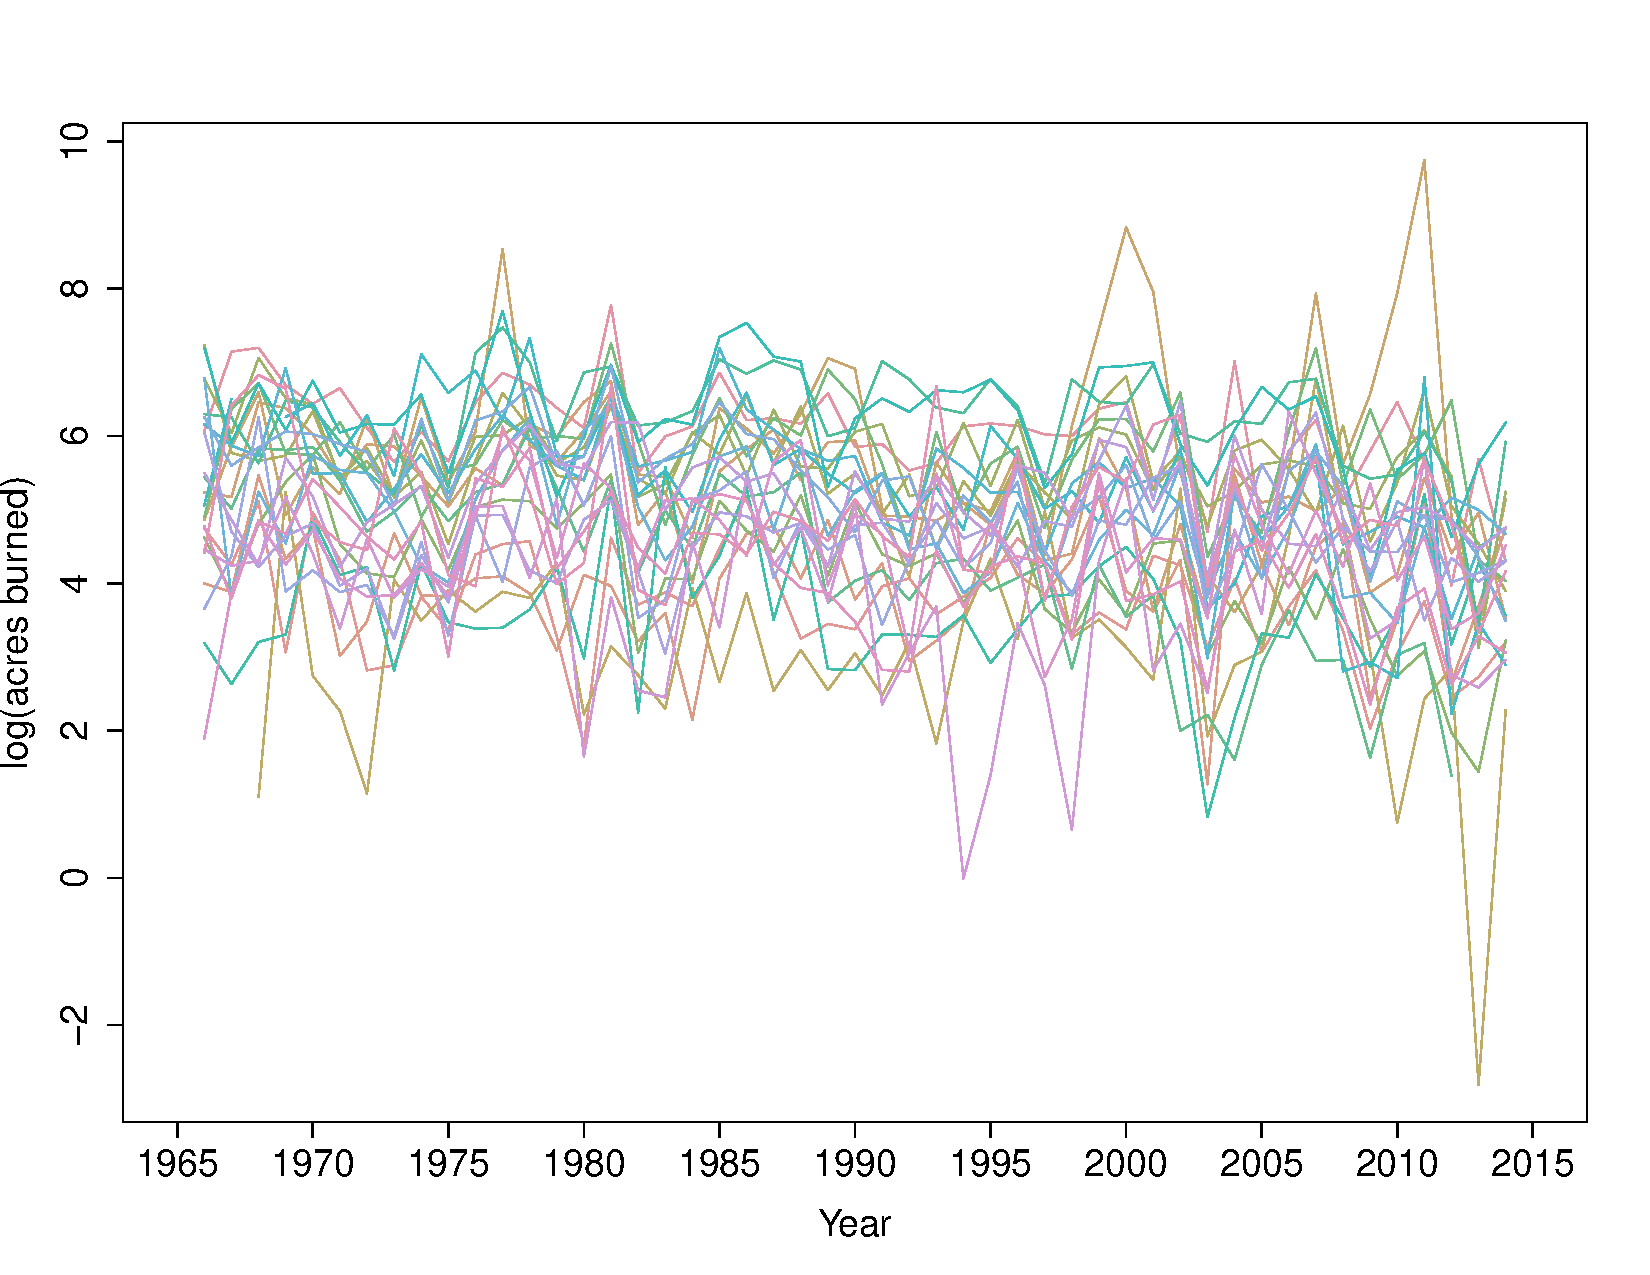
\includegraphics[width=0.60\linewidth]{plots/spag-rand-25}
      \caption{Time series of $\log$(acres burned) for 25 randomly selected counties.}
      \label{fig:firets25}
    \end{figure}
  \end{itemize}
\end{frame}

\begin{frame}{Data application}
\begin{columns}[c]
  \column{.45 \linewidth}
  \begin{itemize} \setlength{\itemsep}{1em}
    \item Data are not max-stable, so we use a site-specific threshold
    \item Threshold originally selected using a spatially smoothed $\hat{q}(0.95)$
  \end{itemize}

  \column{.55 \linewidth}
  \begin{figure}[htbp]
      \centering
      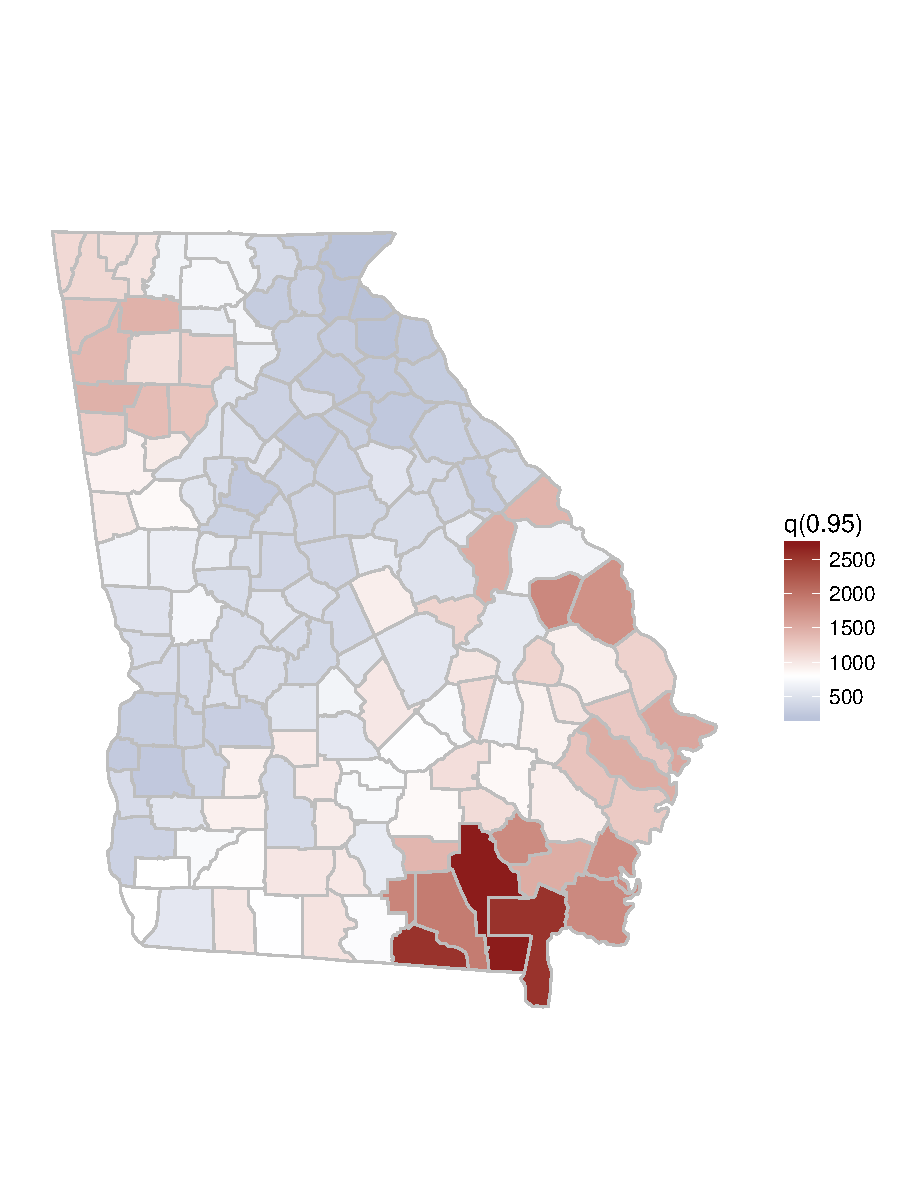
\includegraphics[width=0.8\linewidth, trim = 0 10em 0 0 ]{plots/spatial-q95}
      \caption{Spatially smoothed $\hat{q}(0.95)$}
      \label{fig:thresh}
    \end{figure}
\end{columns}
\end{frame}

\begin{frame}{Analysis}
  \begin{itemize} \setlength{\itemsep}{1em}
    \item Spatio-temporal model for GEV parameters including a linear time trend and interaction with basis functions
    \begin{itemize} \setlength{\itemsep}{0.5em}
      \item $\mu(\bs, t) = \beta_{0, \mu} + \beta_{1, \mu} t + \gamma_{1, \mu} B_1 + \cdots \gamma_{L, \mu} B_L + \delta_{1, \mu} B_1 t + \cdots \delta_{L, \mu} B_L t$
      \item $\log(\sigma) (\bs, t) = \beta_{0, \sigma} + \beta_{1, \sigma} t + \gamma_{1, \sigma} B_1 + \cdots \gamma_{L, \sigma} B_L + \delta_{1, \sigma} B_1 t + \cdots \delta_{L, \sigma} B_L t$
      \item $\xi$ is constant across space
    \end{itemize}
    \item Prior distributions:
    \begin{itemize} \setlength{\itemsep}{0.5em}
      \item $\mu(\bs, t)$: coefficients $\iid N(0, \sigma^2_\mu)$
      \item $\log(\sigma)(\bs, t)$: coefficients $\iid N(0, \sigma^2_\sigma)$ \vspace{0.5em}
      \item $\xi \sim N(0, 0.25)$
    \end{itemize}
    \item Independent IG(0.1, 0.1) priors on $\sigma^2_\mu$ and $\sigma^2_\sigma$
  \end{itemize}
\end{frame}

\begin{frame}{Model comparisons}
  \begin{itemize} \setlength{\itemsep}{1em}
    \item Comparing two different spatial process constructions
    \begin{itemize} \setlength{\itemsep}{0.5em}
      \item Extremal coefficient basis functions (ECB)
      \item Gaussian kernel basis functions (GKB)
    \end{itemize}
    \item Comparing two basis function structures for marginal distributions
    \begin{itemize} \setlength{\itemsep}{0.5em}
      \item Extremal coefficient basis functions (ECB)
      \item 2-dimensional B splines (2BS) (\alert{in progress})
    \end{itemize}
    \item Considering $L = 4, 9, 16, 25$ knots
    \begin{itemize} \setlength{\itemsep}{0.5em}
      \item When $L = 4$ for 2BS, we use a 2nd order spatial model for $\mu(\bs, t)$ and $\log(\sigma) (\bs, t)$
    \end{itemize}
  \end{itemize}
\end{frame}

\begin{frame}{2d B splines}
  \begin{figure}
    \centering
    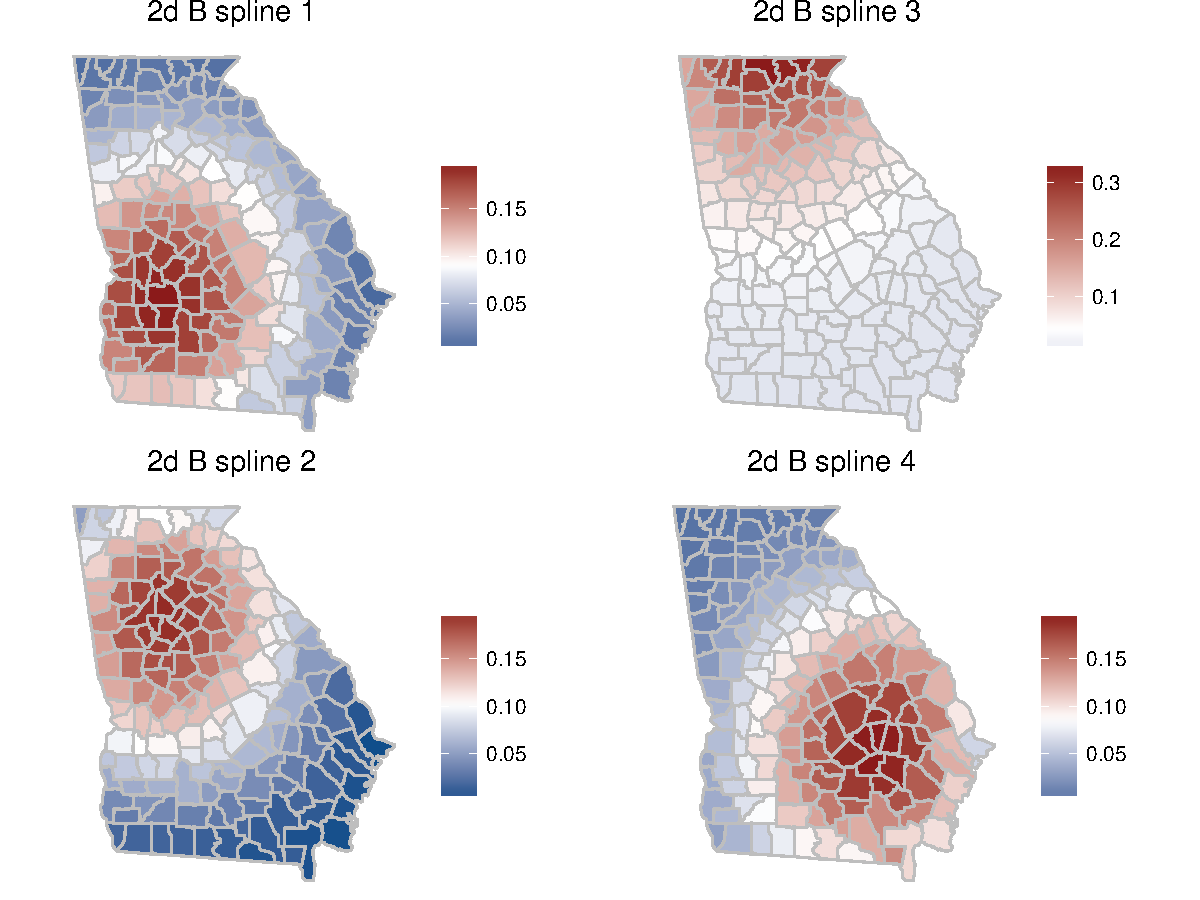
\includegraphics[width = 0.75\linewidth, trim = 0 2em 0 0]{plots/2d-basis.pdf}
    \caption{Four 2-dimensional B splines with $L =$9}
  \end{figure}
\end{frame}

\begin{frame}{Results}
  \begin{figure}  % markdown/fire-analysis/combine-tables.R
    \centering
    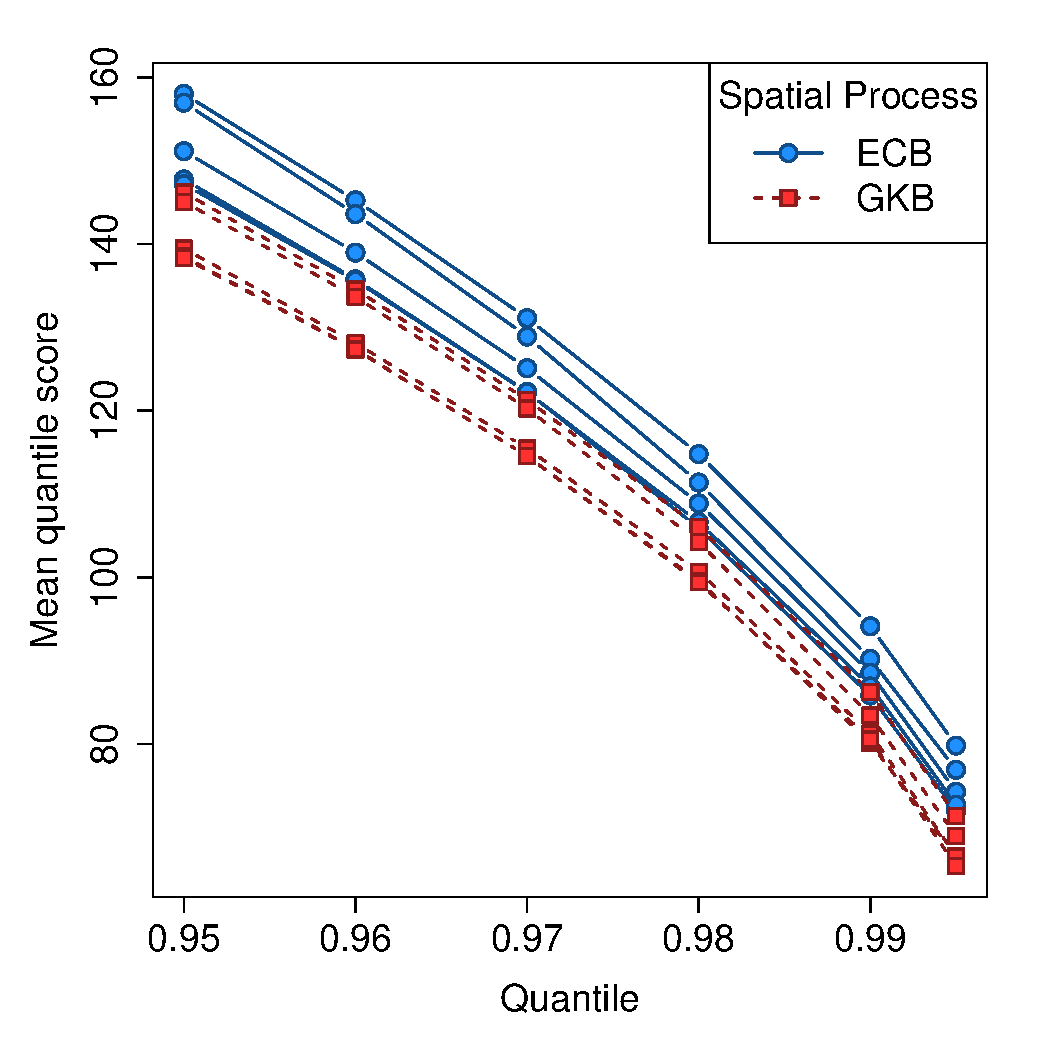
\includegraphics[width=0.47\linewidth]{plots/qs-mean}
    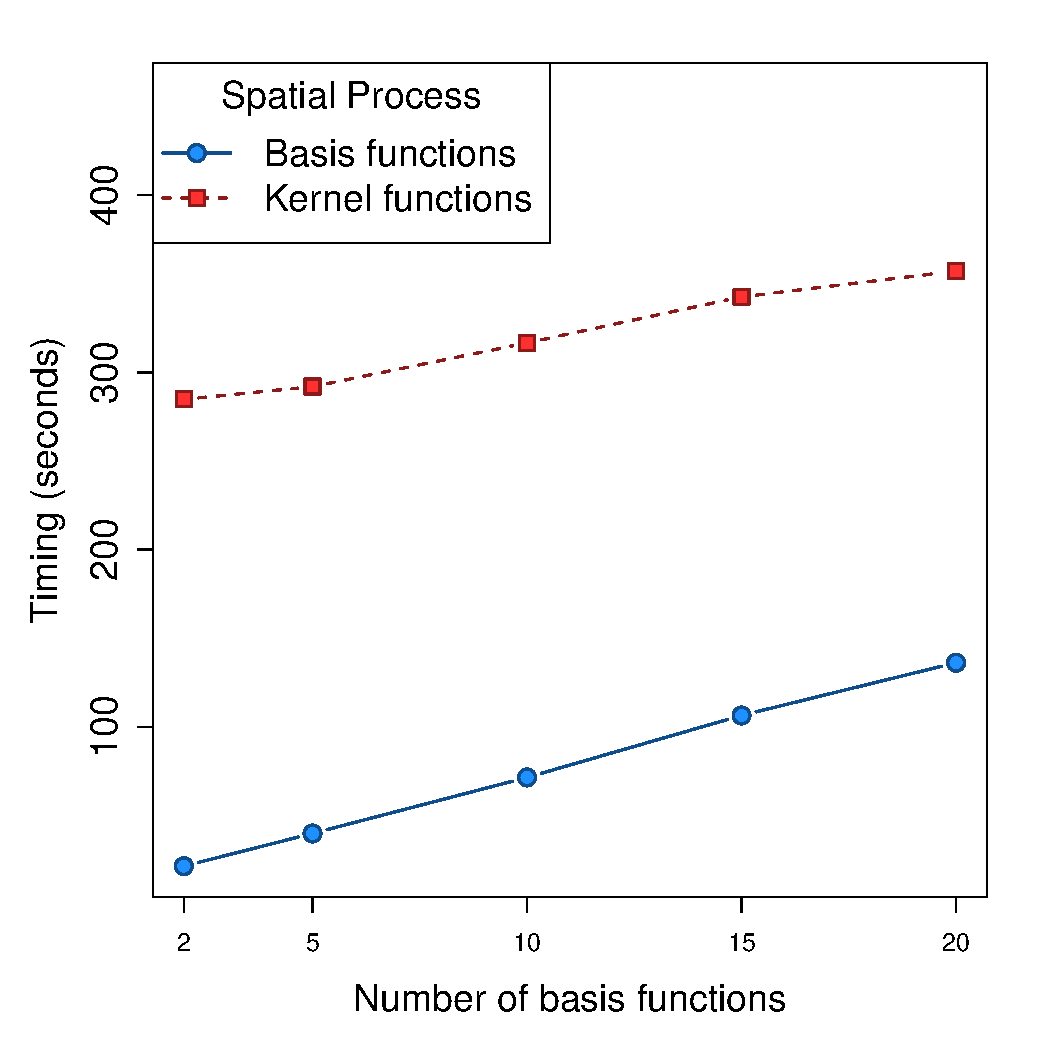
\includegraphics[width=0.47\linewidth]{plots/timing}
    \caption{Average quantile score for selected quantiles and timing comparisons}
    \label{fig:avgqscore}
  \end{figure}
\end{frame}

\begin{frame}{Remaining questions}
  \begin{itemize} \setlength{\itemsep}{1em}
    \item What's the best way to select the threshold for this application?
    \begin{itemize} \setlength{\itemsep}{0.5em}
      \item Mean residual plots are helpful, but can be challenging since not all sites have same marginal parameters
      \item Cross-validation is time intensive
    \end{itemize}
    \item Are there better options for the spatial aspect of the marginal parameters?
    \item Are there better ways to pick the number of knots?
    \begin{itemize}\setlength{\itemsep}{0.5em}
      \item Potentially add knots until the smallest $v_l$ is less than some threshold
    \end{itemize}
  \end{itemize}
\end{frame}

\end{document}